\section{问题一建模}

在问题一中,我们的任务是对视频中出现车辆的15个指标进行检测识别并记录,需要用到计算机视觉的算法。主要有两类任务,一是对数字进行识别,主要是对时间和红绿灯秒数的识别,二是对车辆进行检测。此外还要将图片中的像素距离变换为实际距离。

\subsection{图像识别}

\subsubsection{时间识别}

在本题中,时间的识别包含两个部分,一个是视频左上角的时刻,一个是信号灯倒计时的秒数。我们采用传统的数字图像处理和深度学习相融合的方法进行识别,当两种方法出现不一致的情况时,我们再人工介入,事实证明,我们几乎不需要人工介入。

传统的数字图像处理方法:由于每个摄像头的拍摄位置和角度是固定不变的,因为我们人为地框定需要识别的数字的位置。识别过程如图\ref{fig:digits}所示,我们先将 RGB 三通道的图像转成单通道的灰度图,如果数字为黑色,则我们反转一下,将数字变为白色,如果数字原本就是白色就不需要反转。随后,我们将图像黑白化,色值低于100的像素全部变成0,即黑色,色值大于100的像素全部变成255,即白色。最后,将图像与上一帧的图像作差,如果出现白色块的数量大于设定的阈值(100),则判定数字有变动。

传统的数字图像处理方法只能判断数字是否有变动,但如果时间出现乱码卡顿,或者跳秒的情况,这种方法就不适用了。因此我们引入了深度学习的方法,传统的数字图像处理的方法仅是辅助。我们使用手写数字数据集 MNIST 训练了 Resnet18 网络,并采用半监督学习的方式让预训练的 Resnet18 网络再学习时间数字和红绿灯数字的特征。这样 Resnet18 网络就能比较完美地识别出数字。当两种方法出现矛盾时,我们再人工介入识别。

\begin{figure}[h]
    \centering
    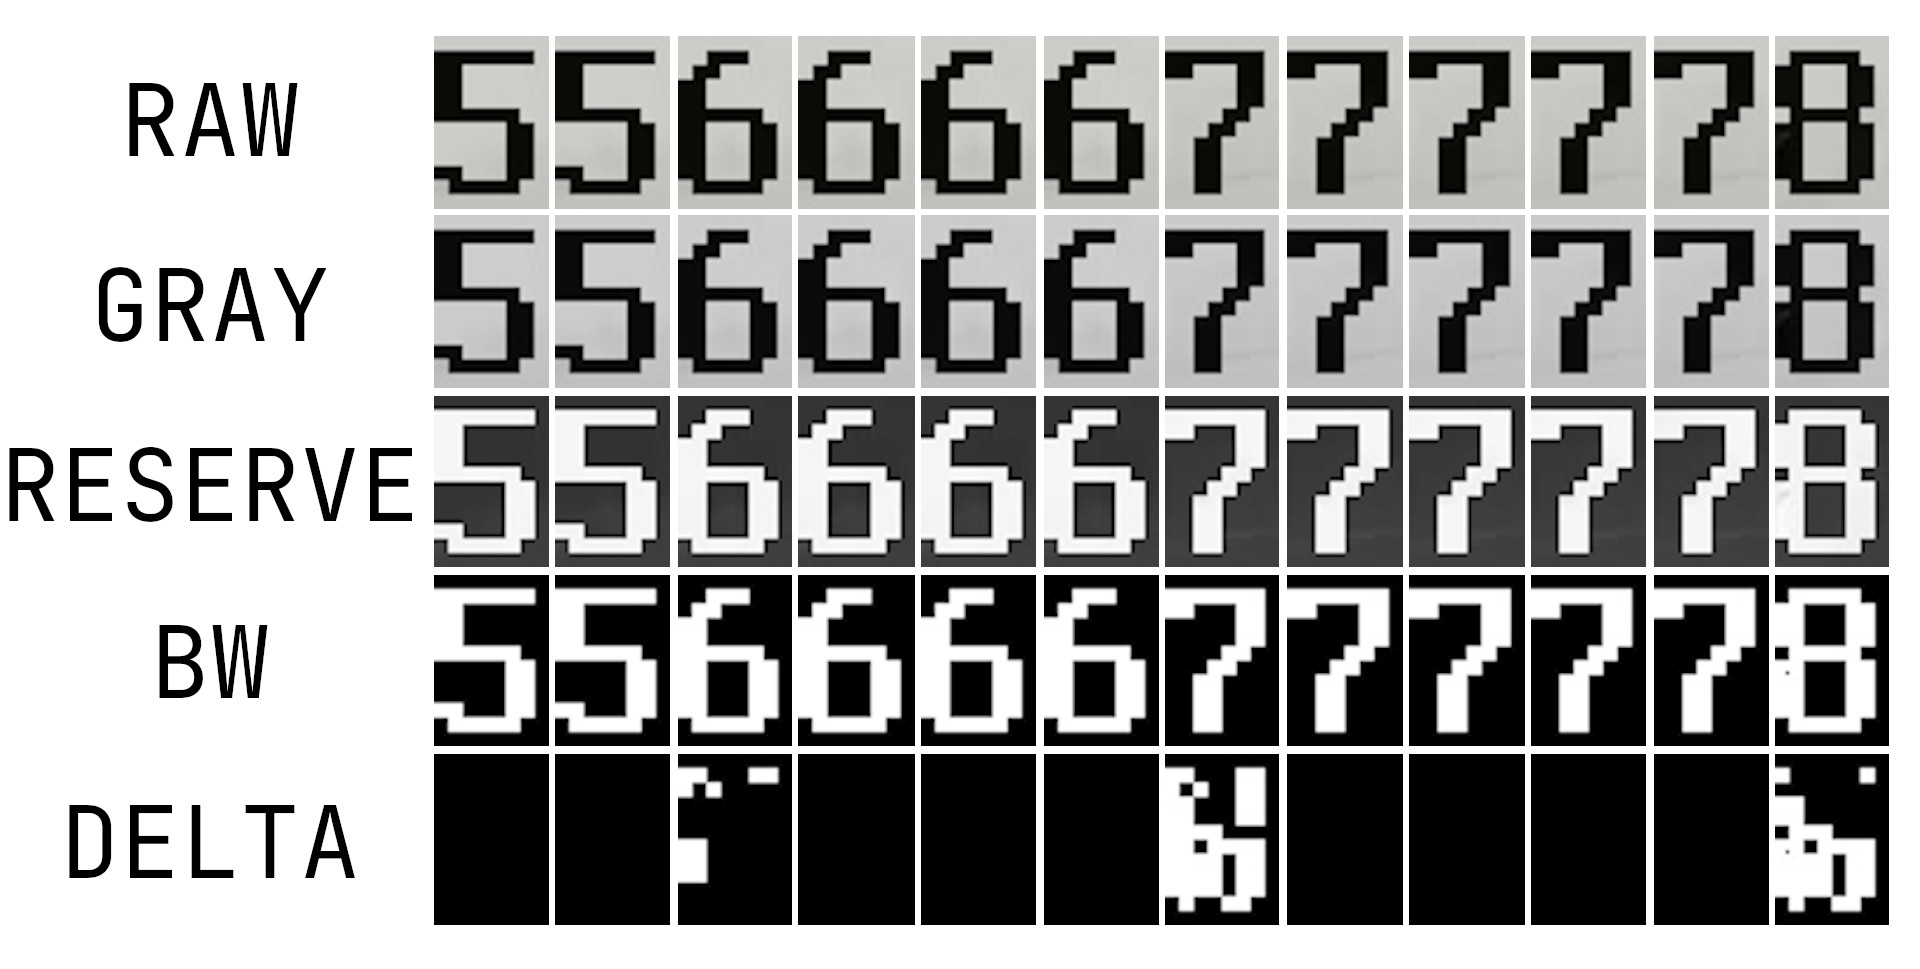
\includegraphics[scale=0.5]{figures/digits}
    \caption{数字变动识别过程}
    \label{fig:digits}
\end{figure}

\subsubsection{车辆检测-YOLO算法}

我们使用 YOLO v3 网络进行车辆检测,YOLO 网络是目前性能比较优秀的一个深度神经网络,经常用于目标检测任务。如\ref{fig:YOLO}所示,YOLO的CNN网络将输入图像分为$S\times S$个网格,每个格子负责检测中心点落在该格子内的目标。若某个物体的中心位置的坐标落到了某个格子,如格点图所示,狗的中心位置位于左下方格点处,那么这个格子就负责检测出这个物体。每个单元格会预测B个边界框以及边界框的置信度。置信度包含两个方面的信息,即边界框含有目标的可能性的大小和边界框的准确度。前者记为$Pr(object)$,若边界框不含物体取值为0,完整包含物体取值为1.准确度信息是用边界框与物体真实区域的交集面积(该面积以像素为单位),记为$IUO^{truth}_{pred}$。置信度的最终定义为$Pr(object)*IUO^{truth}_{pred}$。

边界框的大小和位置可以用4个值来表示(x,y,w,h)。其中(x,y)是边界框的中心坐标,(w,h)是边界框的宽与高。其中(x,y)是相对于每个单元格左上角坐标点的偏移值,并且单位是相对于单元格大小的,边界框的宽和高是相对于整个图片的宽和高的比例,故四个元素的大小应该 均在[0,1]范围内。同时每一个单元格需要预测出C个类别概率值,由该单元格负责的边界框其目标属于各个类别的概率。每个单元格的预测需要$(B*5+C)$个值,如果将输入图片划分成$S*S$网格,那么最终的预测值为$S*S*(B*5+C)$大小的张量。

\begin{figure}[H]
    \centering
    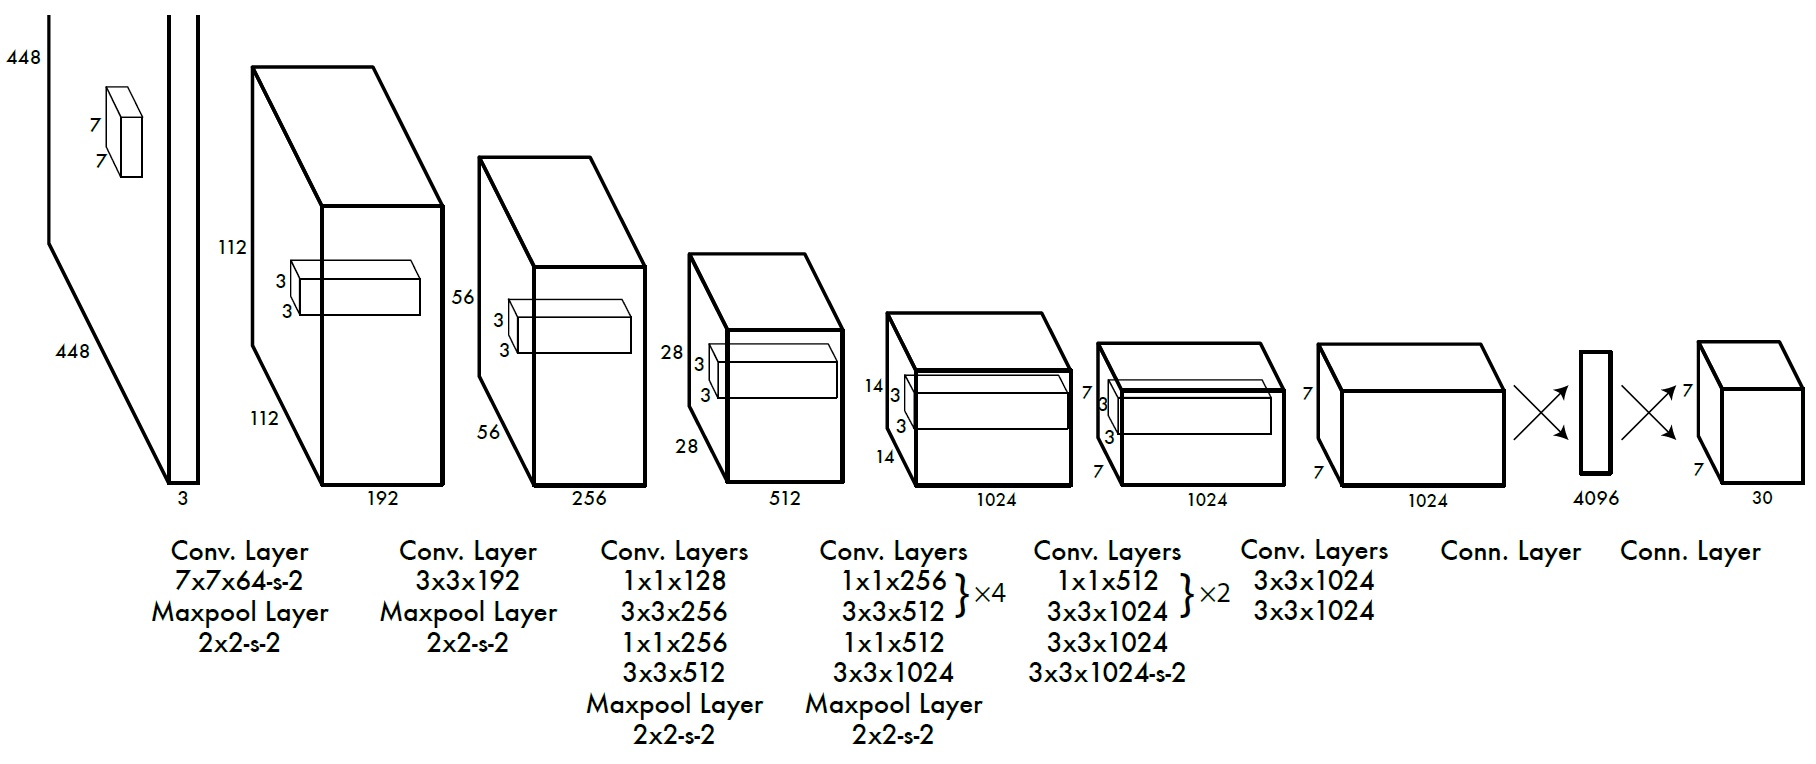
\includegraphics[scale=0.1]{figures/网络结构.jpg}
    \caption{网络结构示意}
    \label{fig:网络}
\end{figure}

Yolo采用卷积提取特征,使用全连接层得到预测值。具体形式可参考下图\ref{fig:网络},如图所示,对于卷积层,主要使用$1 \times 1$卷积来做channle reduction,然后紧跟$3 \times 3$卷积。对于卷积层和全连接层,采用Leaky ReLU激活函数:$max(x,0.1x)$,最后一层采用线性激活函数。YOLO将目标检测看成回归问题,采用的是均方差损失函数。但对不同的部位采用了不同的权重值。定位误差即边界框坐标预测误差的权重值为5;不包含目标的边界框的置信度权重值为0.5;含有目标的边界框的置信权重为1。实际上较小的边界框坐标误差应该比大的边界框更敏感。为了保证这一点,将网络的边界框的宽与高预测改为对其平方根的预测,即预测值变为$(x,y,{\sqrt{w}},\sqrt{h})$,损失函数为:

\begin{equation}
    \begin{aligned}
        &\lambda_{\text {coord }} \sum_{i=0}^{S^{2}} \sum_{j=0}^{B} \mathbb{1}_{i j}^{\text {obj }}\left[\left(x_{i}-\hat{x}_{i}\right)^{2}+\left(y_{i}-\hat{y}_{i}\right)^{2}\right] \\
        &\qquad \begin{aligned}
                    +\lambda_{\text {coord }} \sum_{i=0}^{S^{2}} \sum_{j=0}^{B} \mathbb{1}_{i j}^{\text {obj }}\left[\left(\sqrt{w_{i}}-\sqrt{\hat{w}_{i}}\right)^{2}+\left(\sqrt{h_{i}}-\sqrt{\hat{h}_{i}}\right)^{2}\right] \\
                    +\sum_{i=0}^{S^{2}} \sum_{j=0}^{B} \mathbb{1}_{i j}^{\text {obj }}\left(C_{i}-\hat{C}_{i}\right)^{2} \\
                    +\lambda_{\text {noobj }} \sum_{i=0}^{S^{2}} \sum_{j=0}^{B} \mathbb{1}_{i j}^{\text {noobj }}\left(C_{i}-\hat{C}_{i}\right)^{2} \\
                    +\sum_{i=0}^{S^{2}} \mathbb{1}_{i}^{\text {obj }} \sum_{c \in \text { classes }}\left(p_{i}(c)-\hat{p}_{i}(c)\right)^{2}
        \end{aligned}
    \end{aligned}
\end{equation}

其中第一项是边界框中心坐标的误差,第二项是边界框的高与宽的误差项,第三项是包含目标的边界框的置信度的误差项。通过该算法,我们可以得到包含目标物体的框,并且有标注-car truck-person等信息。

\subsection{距离转换}

\subsubsection{基于相机模型的坐标简介}

相机的拍摄实际上是一个透视过程,在本文的研究中我们用小孔成像模型来研究相机成像。

从计算机视觉的视角,一张图片我们需要考虑多个坐标系:

(1)以相机光心O组成的坐标系称为相机坐标系$O_c-X_c-Y_c-Z_c$;X轴与Y轴分别平行于图像坐标系的X轴和Y轴,Z轴为相机的光轴方向。

(2)以光心在相平面投影$O'$(图像平面中心)为原点的坐标系称为图像坐标系$O-X-Y$;

(3)以图像左上角为原点的坐标系称为像素坐标系$O-u-v$;像素坐标系的两轴分别平行于图像平面的两条垂直边。

(4)物体在真实世界的坐标用世界坐标系来描述$O_w-X_w-Y_w-Z_w$.
我们在博客中找到了下图,可以清晰的表示坐标系间的关系:

\begin{figure}[h]
    \centering
    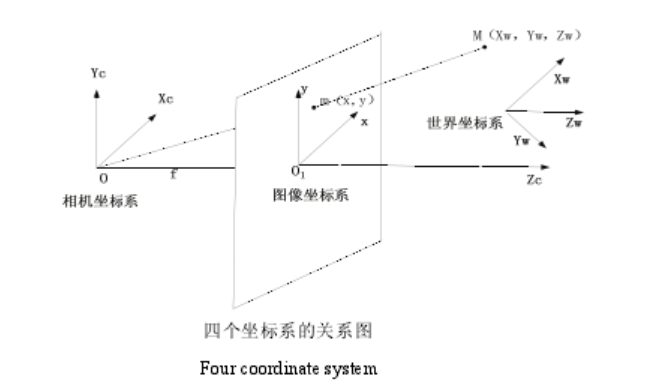
\includegraphics[scale=1]{figures/坐标系相互关系.png}
    \caption{坐标系相互关系}
    \label{fig:p5}
\end{figure}

\subsubsection{相机成像的性质}

在现实生活中,平行的线永不相交,但在照片中,平行的马路不再平行,看似会在远处交于一点,所以照片中的数据性质需要重新进行研究,图像坐标系下的部分距离信息与世界坐标系下并不相一致。

性质1:摄像头把平行的直线映射为图像上的相交直线,这个交点被称为消隐点(vanish point)。所有的平行的直线都各自交于无穷远处的一点,这些点会构成无穷远直线,这条线被称为plane vanishing line-消失的地平线。

\begin{figure}[h]
    \centering
    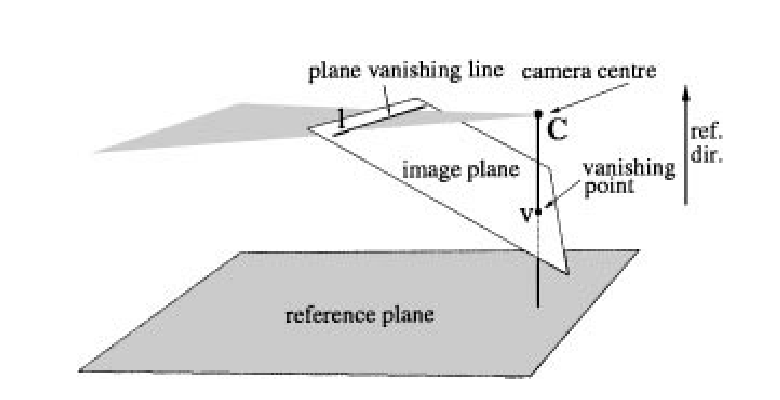
\includegraphics[scale=1]{figures/相机成像.png}
    \caption{相机成像}
    \label{fig:p6}
\end{figure}

这一图片来自论文\cite{2000Single},其中reference plane代表地面,image plane则是相机所拍出的照片,C点为相机的中心点。消失的地平线是由过C点且与地面平行的平面与照片的交线。

性质2:摄像头把三维空间投影到二维图像上,保持直线交比不变。交比是四个点两两“比例的比例”。如果在三维空间中有一条直线上有4个点,那么它们映射到图片上的四个点后,四个点的交比不变。

\begin{figure}[h]
    \centering
    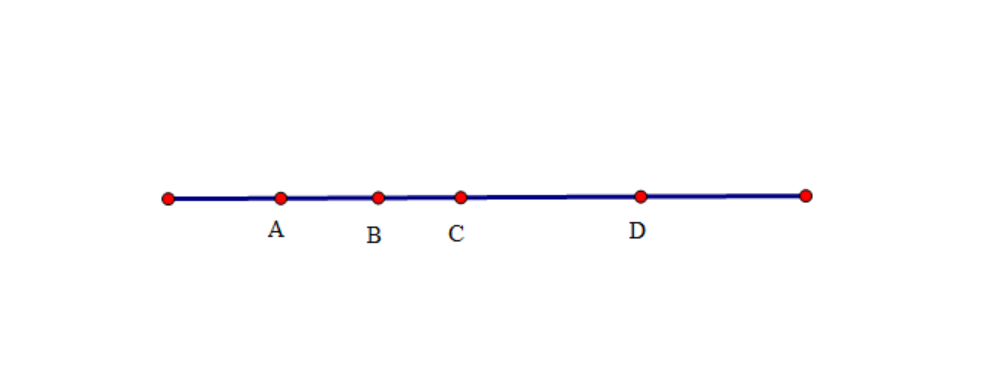
\includegraphics[scale=0.5]{figures/交比示意.png}
    \caption{交比示意图}
    \label{fig:p7}
\end{figure}
此处需要解释一下交比的定义。如图\ref{fig:p7}所示,直线上依次有ABCD四点,那么我们定义四个有序点的交比为:

\begin{equation}
    \frac{CA}{CB}/\frac{DA}{DB}
\end{equation}

\begin{figure}[H]
    \centering
    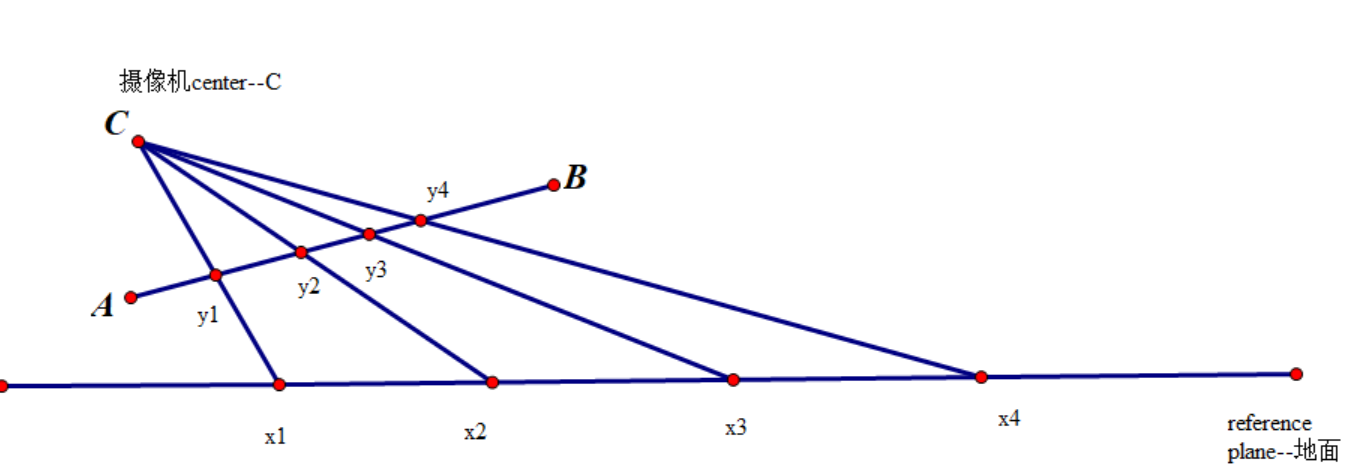
\includegraphics[scale=0.5]{figures/交比不变示意图.png}
    \caption{交比不变示意图}
    \label{fig:p8}
\end{figure}
如\ref{fig:p8}所示,C点为摄像机的中心点,AB可以认为是一张照片,水平线是地面,地面上选取在同一直线上的四个点$x1,x2,x3,x4$,在照片上成像时对应的点为$y1,y2,y3,y4$,交比不变的意思是,有如下等式成立:

\begin{equation}
    \begin{aligned}
        \frac{x3-x1}{x3-x2}/\frac{x4-x1}{x4-x2}=\frac{y3-y1}{y3-y2}/\frac{y4-y1}{y4-y2}
    \end{aligned}
\end{equation}

通过交比不变的性质,我们可以依据图像坐标系中的数据得到世界坐标系下的真实距离。下面我们演示一个例子。以\ref{fig:p4}的北口视频截图为例,计算停车线到图片下沿的长度。

\begin{figure}[H]
    \centering
    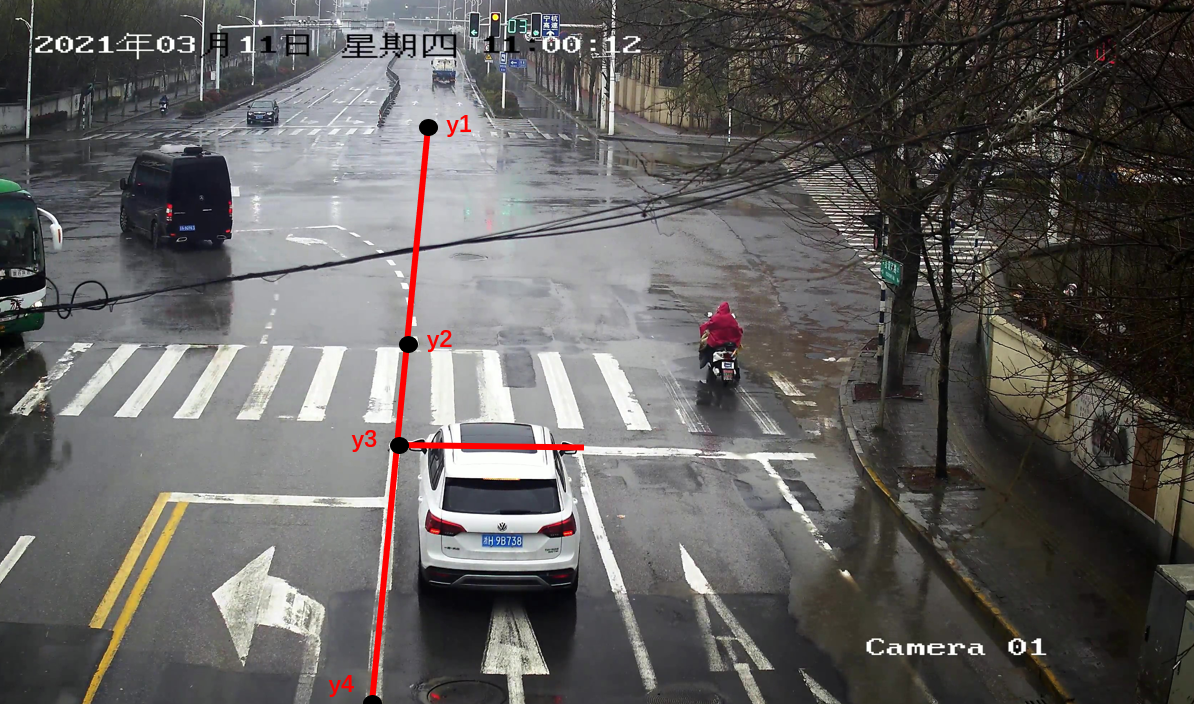
\includegraphics[scale=0.5]{figures/交比示例.png}
    \caption{交比示例}
    \label{fig:交比}
\end{figure}

如\ref{fig:交比}所示,此图为北口示意图,$y1y2$为北口斑马线顶端到南口停车线的图像上长度,$x1x2$为世界坐标系下的真实距离,42米。$y2y3$视为斑马线的图像长度,由于该路口确定,故斑马线长度$x2x3$确定,是3米。$y3y4$是停车线到图片底端的长度,$x3x4$是未知待求的。

\begin{figure}[h]
    \centering
    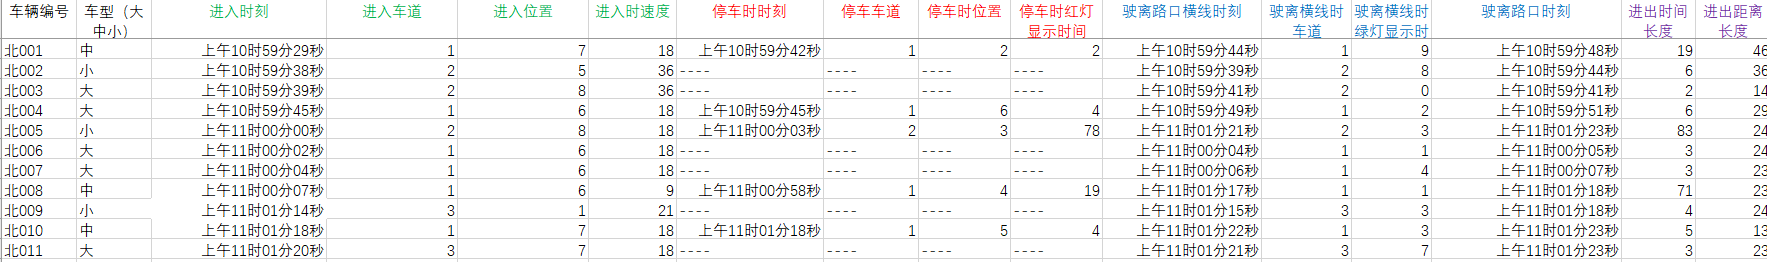
\includegraphics[scale=0.5]{figures/识别结果.png}
    \caption{识别结果}
    \label{fig:识别结果}
\end{figure}

\begin{figure}[h]
    \centering
    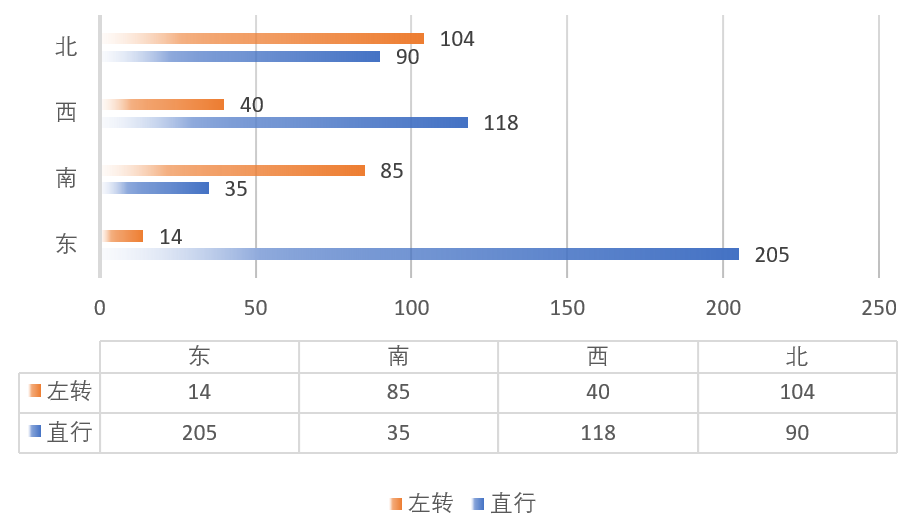
\includegraphics[scale=0.5]{figures/左转直行比例图.png}
    \caption{左转直行比例图}
    \label{fig:左转直行比例图}
\end{figure}

最终我们得到了如图\ref{fig:识别结果}所示结果,有些车的停车四列是虚线表示,代表该车没有等待信号灯,直接行驶了。驶离数据为空的数据行代表在视频周期内,车辆最终未能成功驶离。数据可视化表现为图\ref{fig:左转直行比例图}可以直观的看出东口西口的左转车辆相较南北左转相差悬殊,故二者的左转绿灯时间应该有相应的区别;同时东西的直行相较于南北的直行车辆较多,直行的绿灯应该更长。

\subsection{轨迹链接}
经过上面的处理,我们得到了每一帧图像中包含车辆的所有信息,包括车辆位置、车辆距离、车辆类型等信息。本部分的算法将帧与帧之间进行关联,从而形成完整的车辆轨迹。

图\ref{fig:link} 展示了 Bounding Box 链接的原理图。假设当前帧当前处理的 Bounding Box 是图中蓝色的框,我们需要链接到上一帧的某个 Bounding Box。由于在路口车辆的行驶轨迹肯定是从图像下方到图像上方的,即车辆在路口不能倒车,因此编号为1和2的 Bounding Box 不能链接。而路口车辆轨迹不能左右距离偏差太大,因为我们设置了一个500的水平距离阈值,图中绿色区域是合法的可以链接的区域。3号框由于水平偏移太大,因此不能链接。4、5、6、7号 Bounding Box 是合法的可以被链接的。随后,我们判断所有合法的 Bounding Box 与当前 Bounding Box 的距离,选择距离最小的作为链接框。因此,5号 Bounding Box 是最后的链接的框。

如果一个 Bounding Box 没有可以链接的 Bounding Box,则该框表示有新的车辆进入画面,我们需要新建一条轨迹。考虑到该链接算法的特性,我们在开始遍历 Bounding Box 的时候,需要将所有框的高降序排列(图像上边缘的高为0)。

\begin{figure}[h]
    \centering
    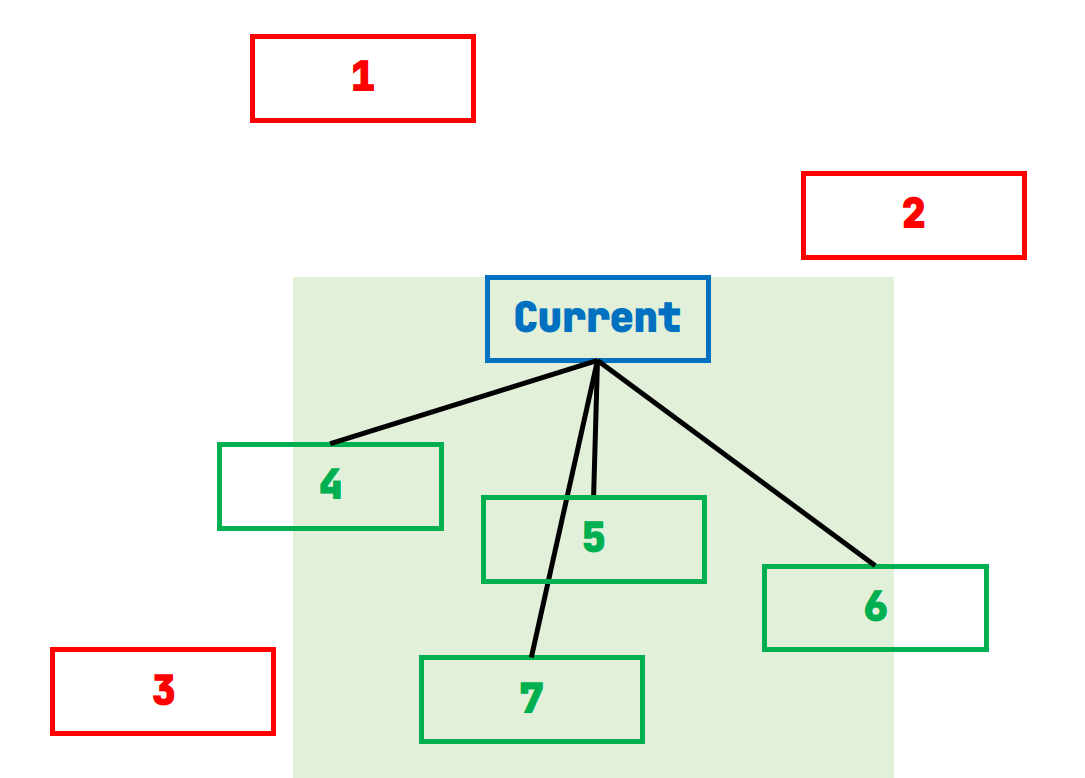
\includegraphics[scale=0.2]{figures/link}
    \caption{Bounding Box 链接原理图}
    \label{fig:link}
\end{figure}

图\ref{fig:demo} 是一段轨迹链接识别的样例,我们以蛇形排列了12帧的图像,这段视频中,链接算法共识别出三辆车的轨迹。某些帧在车辆检测阶段会出现漏检的情况,比如第2帧中红色轨迹的厢式货车,但链接算法具有良好的鲁棒性可以纠正一些错误。

\begin{figure}[h]
    \centering
    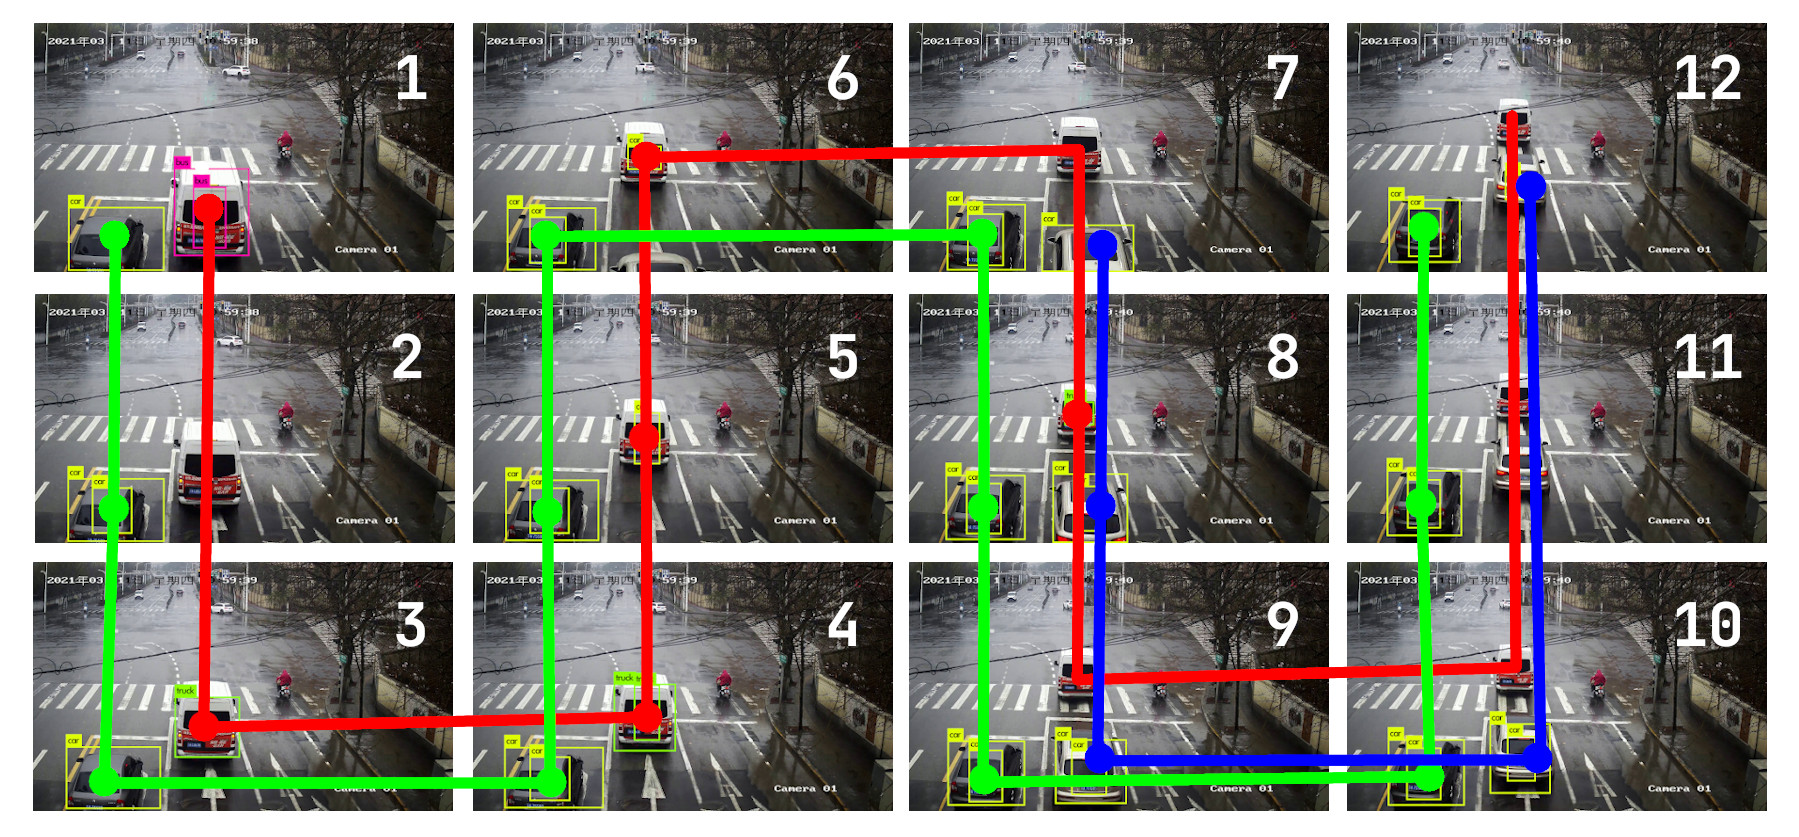
\includegraphics[scale=0.5]{figures/demo}
    \caption{轨迹链接识别示例}
    \label{fig:demo}
\end{figure}
